\section{Ejercicios sobre autómatas finitos y lenguajes regulares}

\begin{problem}[1]
Diseña expresiones regulares para los siguientes lenguajes:
\ppart$L(A) = \lbrace a^nb^m : \ n+m$ es impar $\rbrace$

\ppart Conjunto de números binarios que contienen la subcadena 1010

\ppart Identificadores de un lenguaje de programación que empiezan con el símbolo @, seguido de una letra minúscula y cualquier combinación de letras minúsculas o números.

\solution

\spart
$(aa)*.(a+b).(bb)*$

\spart
$(1+0)*.1010.(1+0)*$

\spart
$@.(a+b+...+z).(0+1+...+9+a+b+...+z)*$
 

\end{problem}


\begin{problem}[2]
Diseña un autómata finito (determinista o no determinista) que reconozca cada uno de los siguientes lenguajes:
\ppart Conjunto de números binarios que contienen la subcadena 1010

\ppart Identificadores de un lenguaje de programación que empiezan con el símbolo @, seguido de una letra minúscula y cualquier combinación de letras minúsculas o números.

\solution
Escojo hacer los diagramas deterministas:\\
\spart
\begin{center}
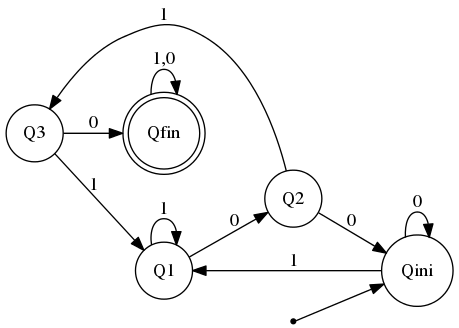
\includegraphics[scale=0.75]{tex/ejerciciosHoja1/automata_2a.png}
\end{center}

\spart
 Las transiciones no indicadas sobreentendemos que van a un nodo residuo.

\begin{center}
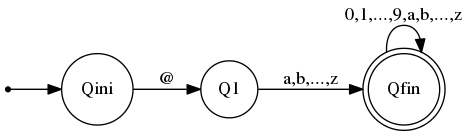
\includegraphics[scale=0.75]{tex/ejerciciosHoja1/automata_2b.png}
\end{center}

 

\end{problem}


\begin{problem}[3]
Indica cuál es el lenguaje aceptado por el siguiente autómata:\\
\begin{center}
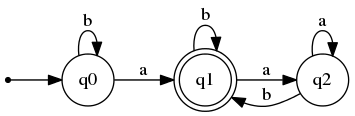
\includegraphics[scale=0.75]{tex/ejerciciosHoja1/automata_3.png}
\end{center}


\solution
Expresión regular: $L(A)=b^*.a+b^*.a.(a+b)^*.b$

Aunque nos pida el lenguaje nos vale con poner la expresión regular.


\end{problem}


\begin{problem}[4]
Construye un autómata finito determinista que acepte cadenas sobre el alfabeto {0,1} que representen números enteros y múltiplos de 5 expresados en representación binaria.

\solution
\begin{expla}
Los estados representan el resto de dividir el número entre 5. Se tiene en cuenta que si tienes un numero cualquiera (por ejemplo 101) al añadirle un 0, es como multiplicarlo por 2, por tanto su resto es el doble, y al añadirle un 1, es como multiplicarle por 2 y sumarle 1.
\end{expla}
\begin{center}
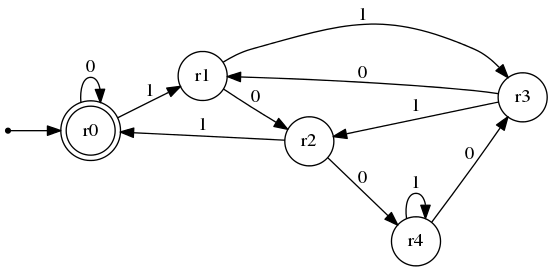
\includegraphics[scale=0.75]{tex/ejerciciosHoja1/automata_4.png}
\end{center}

\end{problem}

 
 \begin{problem}[5]
 Para el autómata siguiente encuentra $\delta^*(q_0,1011)$ y $\delta^*(q_1,01)$ 
 \begin{center}
 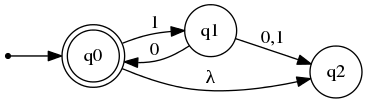
\includegraphics[scale=0.75]{tex/ejerciciosHoja1/automata_5.png}
 \end{center}
 
 \solution
 \begin{expla}
 Nos piden la salida del autómata dada un estado inicial y una palabra.
 \end{expla}
 

 $\delta^*(q_0,1011)$ = q2 \\
 \begin{tabbing}
   \hspace*{2cm} \= \hspace*{2cm} \= \hspace*{2cm} \= \hspace*{2cm} \= \hspace*{2cm} \kill
 Estados \> 1   \> 0   \> 1   \> 1  \\
 q0 \> q1 \> q0 \> q1\> q2  \\
  \>  \> q2 \> - \> -\\
 q2 \> - \> - \> - \> -\\
 \end{tabbing}
 

 $\delta^*(q_1,01)$ = $q1$ \\
  \begin{tabbing}
  \hspace*{2cm} \= \hspace*{2cm} \= \hspace*{2cm} \kill
  Estados \> 0   \> 1  \\
  q1 \> q0 \> q1 \\
   \> q2 \> -\\
  \end{tabbing}
  
 
 \end{problem}
 
 
 \begin{problem}[6]
 Construye un autómata finito no determinista con tres estados que acepte el lenguaje $L=\{ab,abc\}^*$, ¿es posible hacerlo con menos de tres estados?
 
 \solution
 \begin{center}
 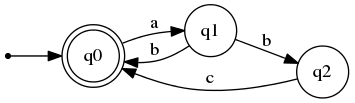
\includegraphics[scale=0.75]{tex/ejerciciosHoja1/automata_6.png}
 \end{center}
  
 
 \end{problem}
 
 \newpage

 
 
 
 
 \section{Ejercicios sobre autómatas a pila y gramáticas independientes del contexto}
 
 \begin{problem}[1]
 Diseña una gramática independiente del contexto que genere el lenguaje de los números capicúa formados con el alfabeto $\Sigma = {0,1,2,3,4,5,6,7,8,9} $. Los números de una sola cifra no se consideran capicúa.
 

 \solution
 
 
  En cada regla, si aparecen dos 'X' estas tienen que acabar en el mismo símbolo terminal. La otra opción era poner muchas reglas más tipo $X_0,...,X_9$.
  
  $S \longrightarrow XZX$
  
  $Z \longrightarrow XZX|X|\lambda$
  
  $X\longrightarrow 0|1|2|3|4|5|6|7|8|9$
 
 \end{problem}
 
 \begin{problem}[2]
 Diseña una gramática independiente del contexto que genere el lenguaje de los números formados con el alfabeto $\Sigma = {0,1,2,3,4,5,6,7,8,9} $ que tengan el mismo número de dígitos pares e impares. Puede suponer por simplicidad que los números pueden tener ceros a la izquierda.
 
 
 \solution
 $S \longrightarrow PSI|ISP|PI|IP|SS$
 
  $P \longrightarrow 0|2|4|6|8$
  
  $I \longrightarrow 1|3|5|7|9$
  
  
 
 \end{problem}
 
 \begin{problem}[3]
Diseña un autómata a piña que reconozca el lenguaje del ejercicio 1.
 
 
 \solution
 \begin{expla}
 Cuando pongo 'x' o 'y' quiero decir un símbolo del conjunto \{0,1,2,3,4,5,6,7,8,9\}. Cuando pongo 'x' e 'y' en la misma transición, $x \neq y$.
 \end{expla}
 \begin{center}
  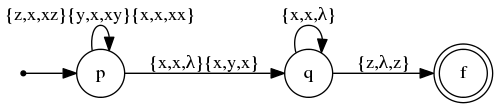
\includegraphics[scale=0.75]{tex/ejerciciosHoja1/automata_7.png}
  \end{center}
 
 \end{problem}
 
 \begin{problem}[4]
 Demuestra que la siguiente gramática es ambigua:
 
 $S \longrightarrow AB | aaB$
 
 $A \longrightarrow a|Aa$
 
 $B\longrightarrow b$
 
 
 \solution
 Si derivamos usando la primera regla de S obtenemos:\\
 $S \longrightarrow AB \longrightarrow AaB \longrightarrow aaB \longrightarrow aab $
 
  Si derivamos usando la segunda regla de S obtenemos:\\
  $S \longrightarrow aaB \longrightarrow aab$
 
 \end{problem}
  
  \begin{problem}[5]
  Encuentra una gramática independiente del contexto para el siguiente lenguaje:\\
  $L=\{a^nww^Rb^n:w\in\{a,b\}^*, n\geq1\}$
  
  \solution
  $w^R$, es la imagen simétrica de la cadena $w$. Si $w$ es $aab$, $w^R$ es $baa$.
  
   $S \longrightarrow aSb | aXb | $
   
   $X \longrightarrow aXa | bXb | \lambda$

  
  \end{problem}
  
  \begin{problem}[6]
  Indica cuál es el lenguaje aceptado por el siguiente autómata a pila:\\
  $A = (\{q_0,q_1,q_2\},\{a,b\},\{a,b,z\},\delta,q_0,z,\{q_2\})$\\
  $\delta(q_0,a,z) = \{(q_1,a),(q_2,\lambda)\} $\\
   $\delta(q_1,b,a) = \{(q_1,b)\} $\\
   $\delta(q_1,b,b) = \{(q_1,b)\} $\\
   $\delta(q_1,a,b) = \{(q_2,\lambda)\} $\\
  
  \solution
  El autómata a pila sería el siguiente:
  \begin{center}
    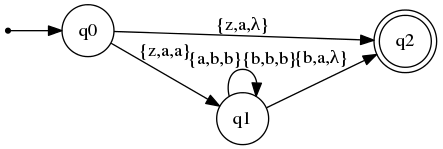
\includegraphics[scale=0.75]{tex/ejerciciosHoja1/automata_8.png}
   \end{center}
   El lenguaje consiste en expresiones del tipo $\{a\}\cup\{ab^n a\\forall n>0\}$
  
  \end{problem}
  
  
  
 
 
 
 
 
 
 
\end{document}
